\documentclass[aspectratio=169, 11pt]{beamer}

\usetheme{metropolis}
\usepackage{amsmath, amssymb, bm}
\usepackage{graphicx}
\usepackage{booktabs}
\usepackage{xcolor}

\graphicspath{{figs/}}

\definecolor{albert}{RGB}{200, 50, 50}
\setbeamercolor{frametitle}{bg=albert!90!black, fg=white}
\setbeamercolor{progress bar}{fg=albert}
\setbeamercolor{alerted text}{fg=albert}

\title{A --- Gradient Descent Regression}
\subtitle{Maths for Machine Learning --- Group Mini-Project}
\author{International MSc Finance \& Data --- Albert School}
\date{2026}

\begin{document}

% ============================================================
\begin{frame}[plain]
  \maketitle
\end{frame}

% ============================================================
\begin{frame}{Outline}
  \tableofcontents
\end{frame}

% ============================================================
\section{Problem \& Dataset}

\begin{frame}{The task}
  \begin{columns}[T]
    \begin{column}{0.55\textwidth}
      \textbf{Goal:} predict house sale prices using linear regression.

      \medskip
      \begin{itemize}
        \item Implement gradient descent \alert{from scratch} (no sklearn).
        \item Tune learning rates, compare convergence.
        \item Benchmark against closed-form OLS.
        \item Explore with PCA and Ridge regression.
      \end{itemize}

      \medskip
      \textbf{Core sessions:} all five (S1--S5).
    \end{column}
    \begin{column}{0.4\textwidth}
      \textbf{Dataset}\\[4pt]
      Kaggle --- Ames Housing\\
      1\,460 houses $\times$ 80 columns\\[6pt]
      Selected \textbf{10 numeric features}:\\
      OverallQual, GrLivArea,\\
      GarageCars, GarageArea,\\
      TotalBsmtSF, 1stFlrSF,\\
      FullBath, TotRmsAbvGrd,\\
      YearBuilt, YearRemodAdd\\[6pt]
      \textbf{Target:} $\log(\text{SalePrice})$
    \end{column}
  \end{columns}
\end{frame}

% ============================================================
\section{Exploratory Data Analysis}

\begin{frame}{Target distribution \& normality (Session 3)}
  \centering
  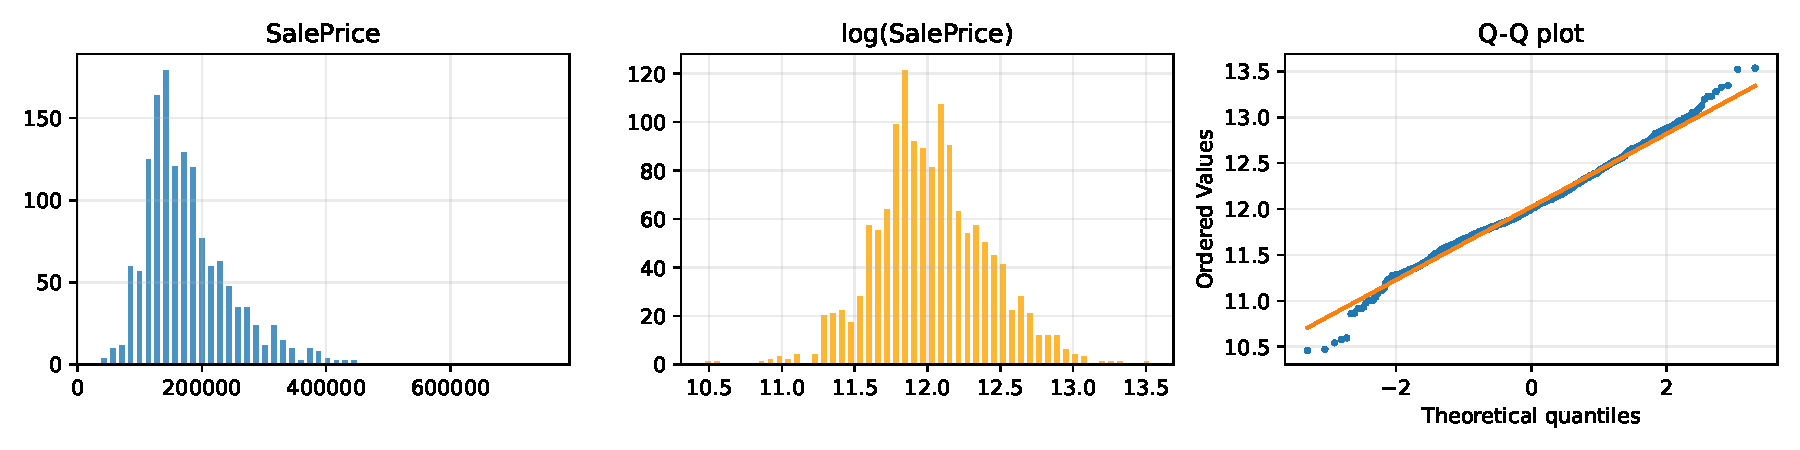
\includegraphics[width=0.78\textwidth]{target_dist.pdf}

  \medskip
  Raw skew $= 1.88 \to$ log skew $= 0.12$. Q-Q plot confirms near-normality.\\
  Shapiro-Wilk $p < 0.05$ but visual improvement is clear --- justifies log-transform for MSE.
\end{frame}

\begin{frame}{Correlation heatmap}
  \begin{columns}[c]
    \begin{column}{0.5\textwidth}
      \centering
      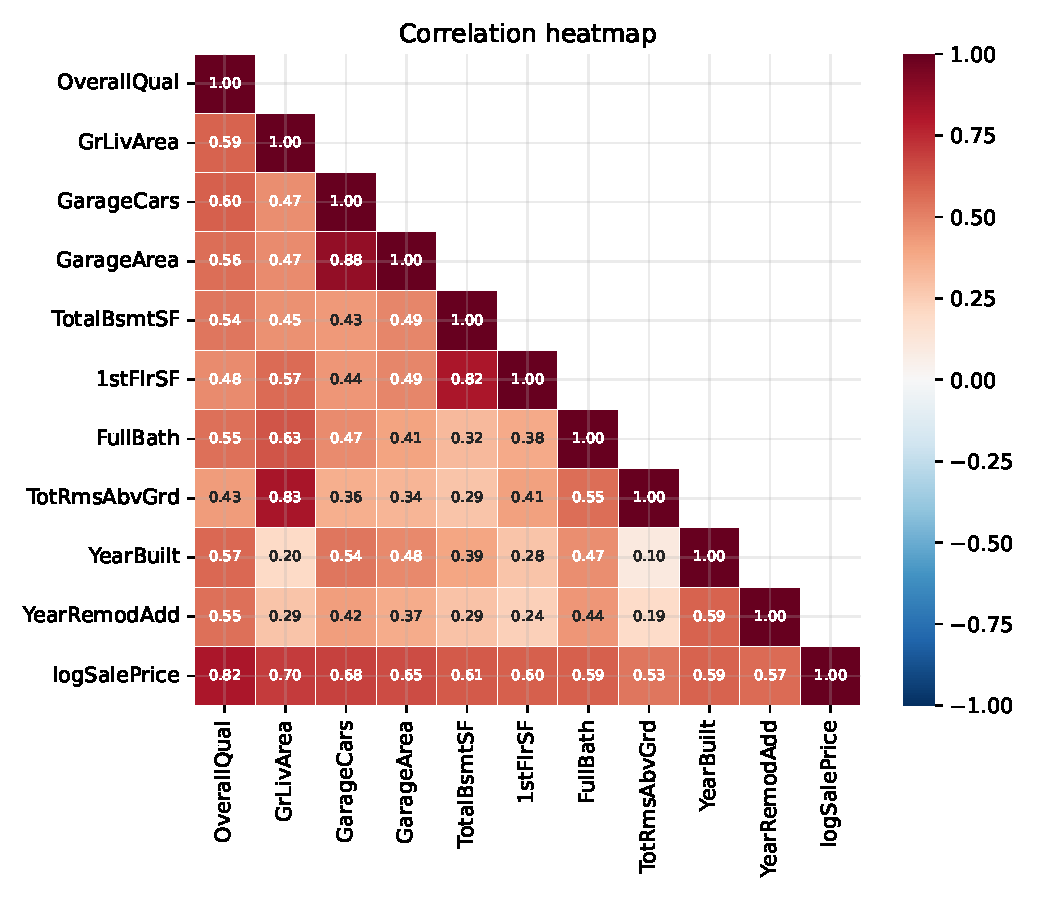
\includegraphics[width=\textwidth]{corr_heatmap.pdf}
    \end{column}
    \begin{column}{0.45\textwidth}
      \textbf{Session 1:} correlation $= \frac{\vec{x}_i \cdot \vec{x}_j}{\|\vec{x}_i\|\|\vec{x}_j\|}$ --- normalised \alert{dot product}.

      \medskip
      Strongest predictors:\\[4pt]
      \begin{tabular}{lr}
        \toprule
        Feature & $r$ \\
        \midrule
        OverallQual & +0.82 \\
        GrLivArea   & +0.71 \\
        GarageCars  & +0.65 \\
        TotalBsmtSF & +0.62 \\
        \bottomrule
      \end{tabular}

      \medskip
      Note: GarageCars/GarageArea are highly correlated ($r=0.88$) --- PCA will handle this redundancy.
    \end{column}
  \end{columns}
\end{frame}

\begin{frame}{Hypothesis test --- does quality matter? (Session 4)}
  \begin{columns}[c]
    \begin{column}{0.52\textwidth}
      \centering
      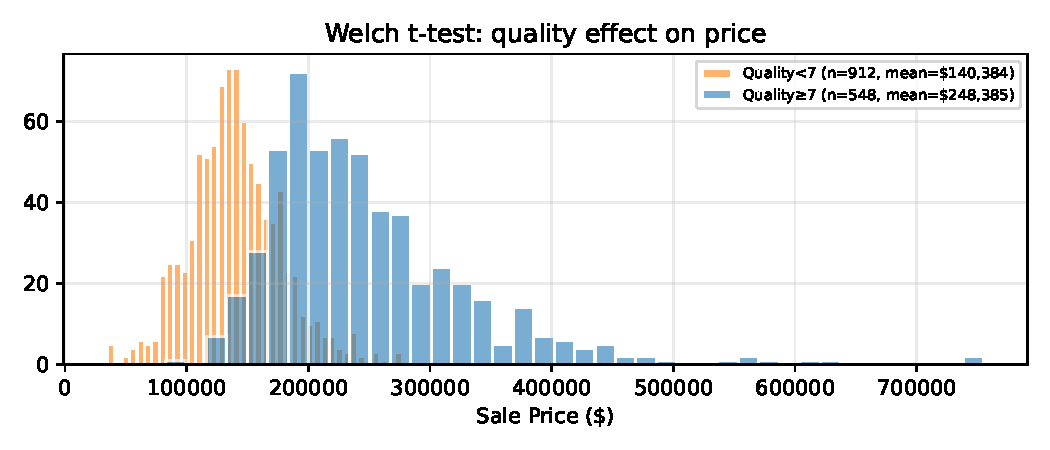
\includegraphics[width=\textwidth]{hypothesis.pdf}
    \end{column}
    \begin{column}{0.43\textwidth}
      \textbf{Welch's $t$-test} (unequal variances):

      \medskip
      $H_0$: $\mu_{\text{high}} = \mu_{\text{low}}$\\
      $H_1$: $\mu_{\text{high}} \neq \mu_{\text{low}}$

      \medskip
      $t = 28.2$,\quad $p \approx 10^{-116}$

      \medskip
      \alert{Reject $H_0$} at $\alpha = 0.05$. \\[4pt]
      OverallQual is a statistically significant predictor --- confirmed by both correlation and hypothesis testing.
    \end{column}
  \end{columns}
\end{frame}

% ============================================================
\section{Mathematical Framework}

\begin{frame}{The model --- Sessions 1 \& 2}
  \textbf{Data as matrix:} $X \in \mathbb{R}^{n \times d}$, each row = one house.

  \medskip
  \textbf{Closed-form OLS} (Session 1 --- matrix inverse):
  \[
    \hat{\beta} = (X^\top X)^{-1}\; X^\top y
  \]

  \textbf{MSE loss} (Session 2 --- gradient descent):
  \[
    \mathcal{L}(\vec{w}) = \frac{1}{n}\|y - X\vec{w}\|^2, \quad
    \nabla_{\vec{w}}\mathcal{L} = \frac{-2}{n} X^\top(y - X\vec{w})
  \]

  \textbf{Update rule:}
  $\vec{w}_{t+1} = \vec{w}_t - \alpha\,\nabla\mathcal{L}(\vec{w}_t)$

  \medskip
  \textbf{Results:} both methods $\to$ Test $R^2 = 0.80$, MSE $= 0.032$
\end{frame}

% ============================================================
\section{Learning Rate \& Convergence}

\begin{frame}{Learning rate sweep}
  \centering
  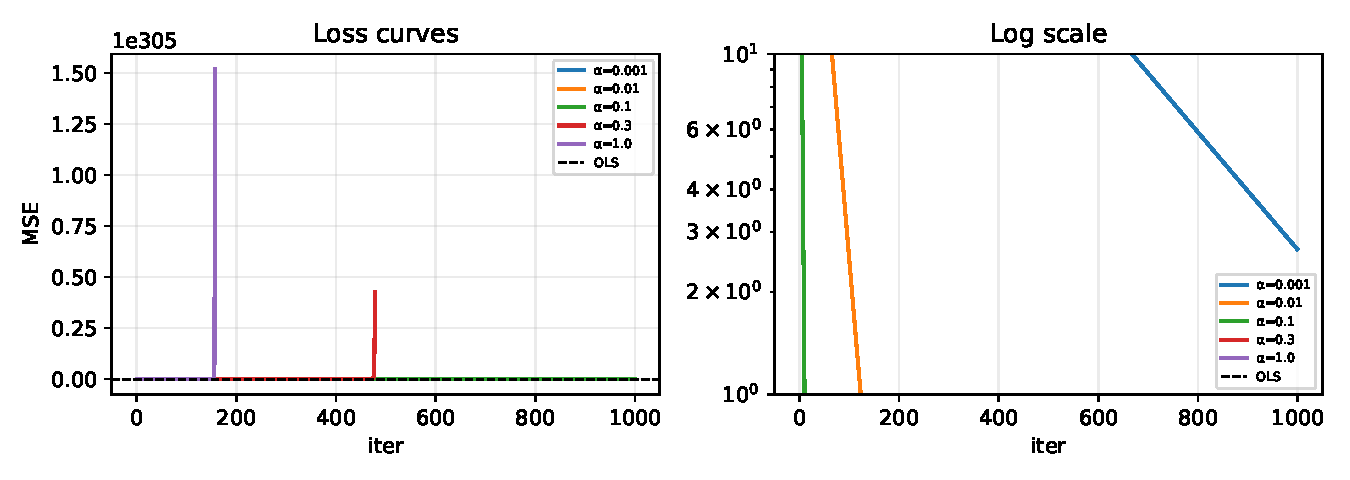
\includegraphics[width=0.78\textwidth]{loss_curves.pdf}

  \medskip
  $\alpha = 0.001$: too slow. \quad $\alpha = 0.01, 0.1$: converge. \quad $\alpha = 0.3, 1.0$: \alert{diverge}.
\end{frame}

\begin{frame}{Gradient norm}
  \centering
  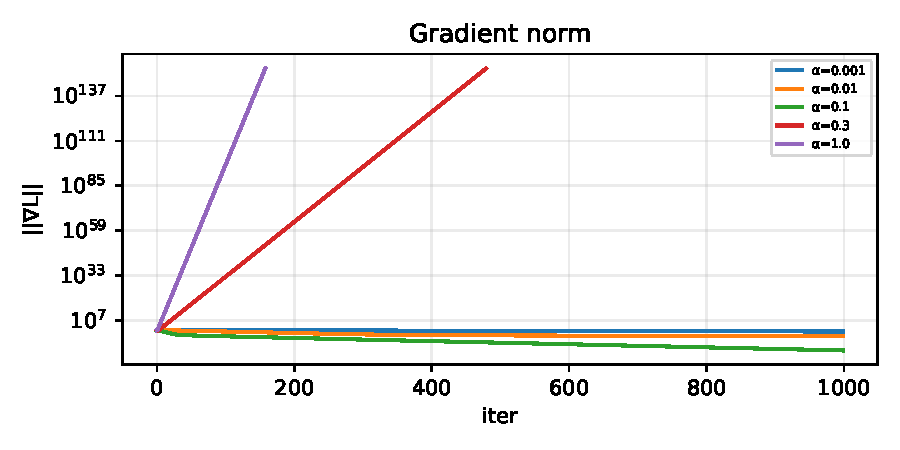
\includegraphics[width=0.55\textwidth]{grad_norm.pdf}

  \medskip
  $\|\nabla\mathcal{L}\| \to 0$ at convergence. For $\alpha \geq 0.3$, it explodes.
\end{frame}

\begin{frame}{Why? The Hessian eigenvalue bound}
  \textbf{Session 1 $\times$ Session 2.} The Hessian is:
  $H = \frac{2}{n} X^\top X$

  \medskip
  Its \alert{eigenvalues} (Session 1) set the curvature. Stability requires:
  \[
    \alpha < \frac{2}{\lambda_{\max}(H)} = \frac{2}{10.27} = 0.195
  \]

  \begin{center}
    \begin{tabular}{lcc}
      \toprule
      & Value & Verdict \\
      \midrule
      $\alpha = 0.1$ & $< 0.195$ & \textcolor{green!60!black}{safe} \\
      $\alpha = 0.3$ & $> 0.195$ & \textcolor{red}{diverges} \\
      $\alpha = 1.0$ & $\gg 0.195$ & \textcolor{red}{diverges} \\
      \bottomrule
    \end{tabular}
  \end{center}

  \medskip
  Condition number $\kappa = 50$ --- standardisation reduced this by orders of magnitude.
\end{frame}

% ============================================================
\section{Visualising Gradient Descent}

\begin{frame}{3D loss surface}
  \centering
  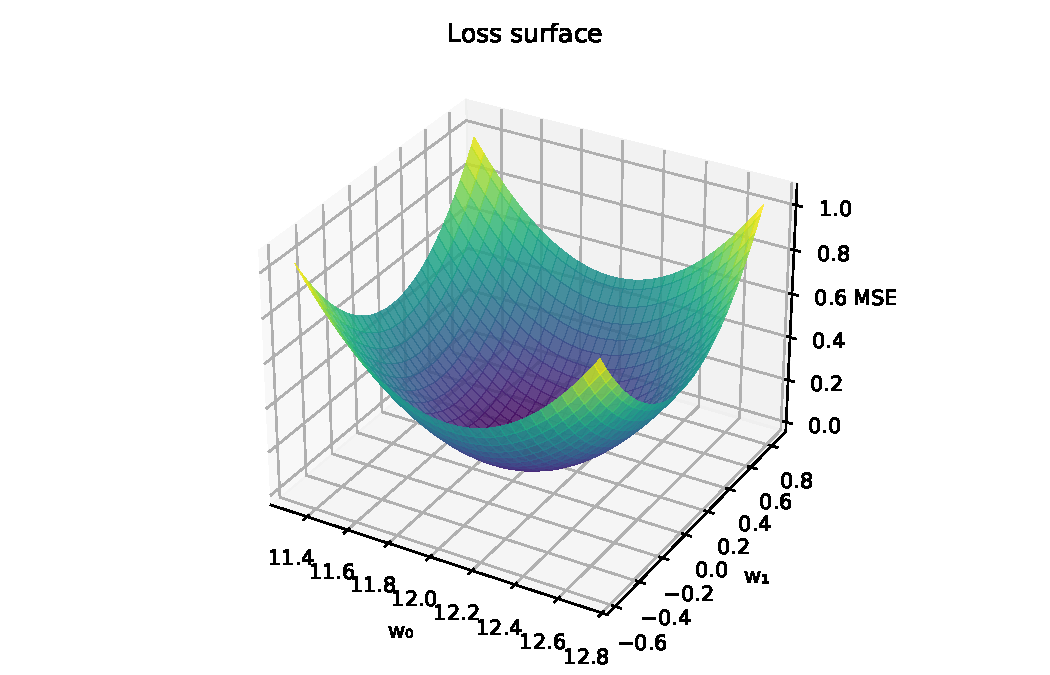
\includegraphics[width=0.55\textwidth]{loss_surface_3d.pdf}

  \medskip
  Slice through $w_0$ (bias) and $w_1$ (OverallQual). MSE is a \alert{convex bowl}.
\end{frame}

\begin{frame}{GD trajectories on contour}
  \centering
  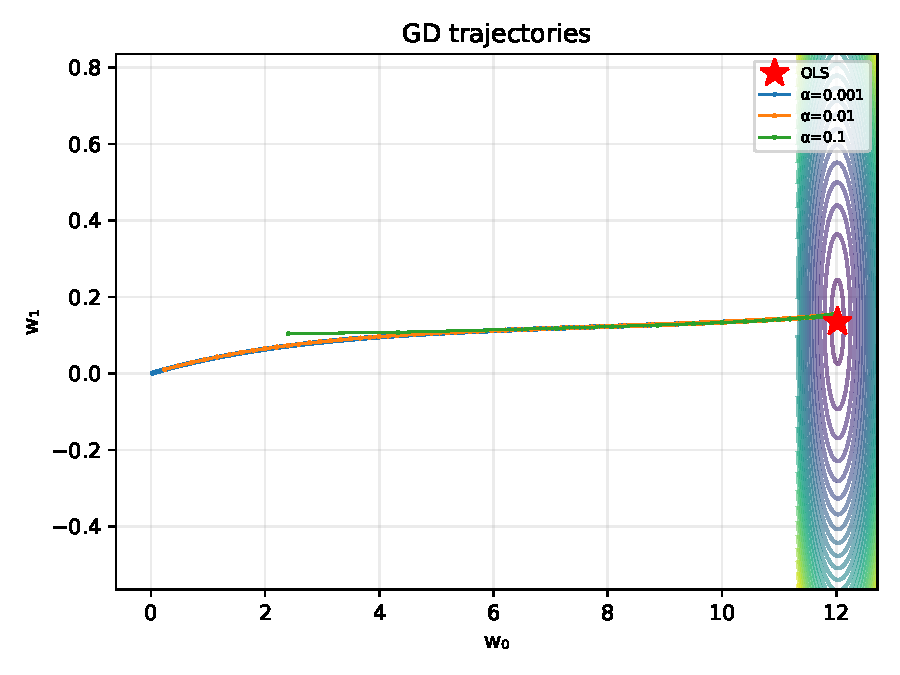
\includegraphics[width=0.5\textwidth]{contour_traj.pdf}

  \medskip
  Paths from $\vec{w}=\vec{0}$ toward the OLS minimum. Larger $\alpha$ = bigger steps.
\end{frame}

% ============================================================
\section{GD Variants \& Comparison}

\begin{frame}{Batch vs Mini-batch vs SGD}
  \centering
  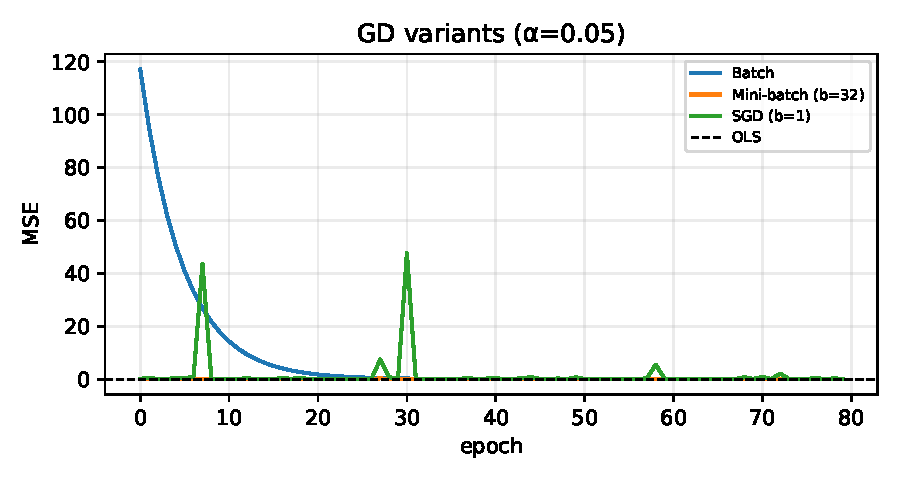
\includegraphics[width=0.52\textwidth]{gd_variants.pdf}

  \medskip
  \begin{tabular}{lcl}
    \toprule
    Variant & Samples/step & Trade-off \\
    \midrule
    Batch     & all $n$ & Exact, slow \\
    Mini-batch & $b=32$  & Balanced \\
    SGD       & $1$      & Noisy, fast \\
    \bottomrule
  \end{tabular}
\end{frame}

\begin{frame}{GD vs OLS --- head-to-head}
  \begin{columns}[c]
    \begin{column}{0.48\textwidth}
      \centering
      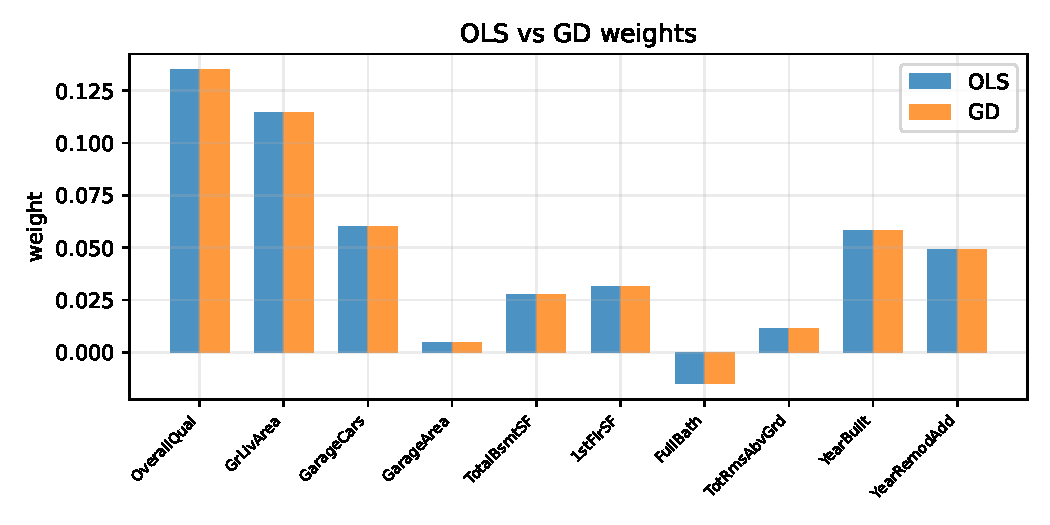
\includegraphics[width=\textwidth]{weight_comparison.pdf}
    \end{column}
    \begin{column}{0.48\textwidth}
      \begin{tabular}{lccc}
        \toprule
        Metric & OLS & GD \\
        \midrule
        Test MSE & 0.032 & 0.032 \\
        Test $R^2$ & 0.802 & 0.802 \\
        $\|\vec{w}_{GD} - \vec{w}_{OLS}\|$ & --- & $10^{-15}$ \\
        \bottomrule
      \end{tabular}

      \medskip
      GD \textit{exactly} recovers OLS to machine precision with a safe $\alpha$.
    \end{column}
  \end{columns}
\end{frame}

\begin{frame}{Test predictions \& residuals}
  \centering
  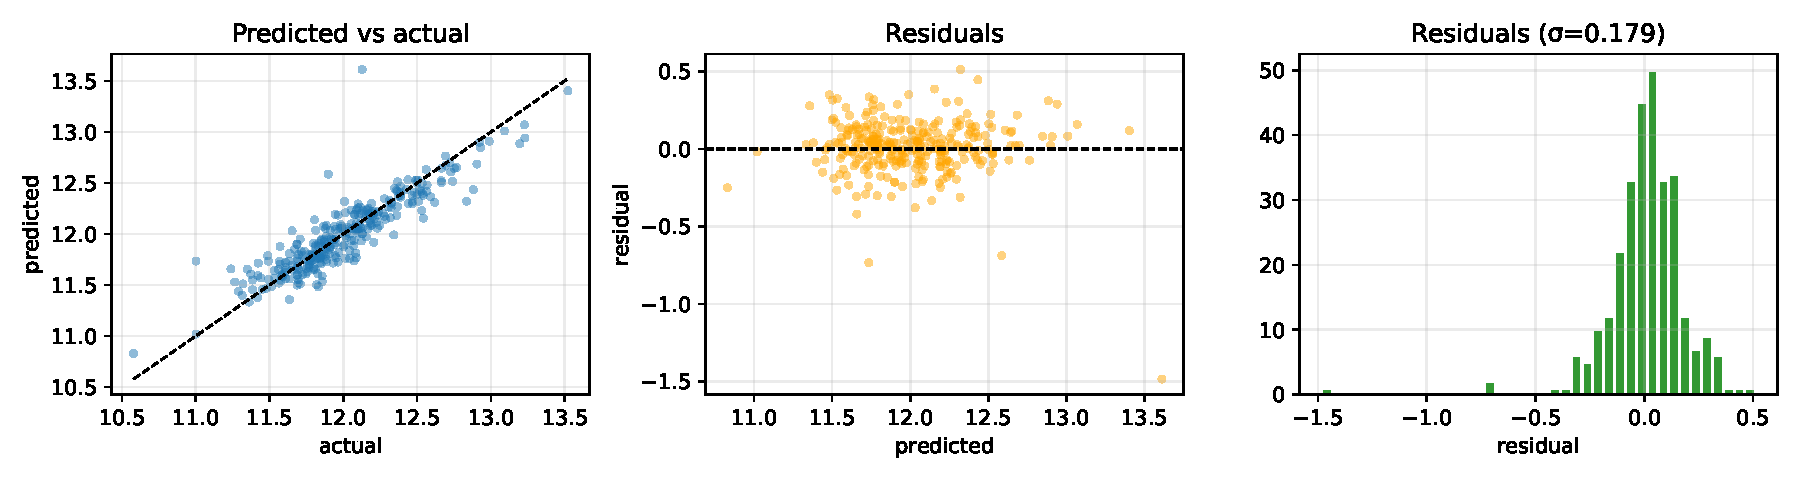
\includegraphics[width=0.82\textwidth]{pred_vs_actual.pdf}
\end{frame}

% ============================================================
\section{Ridge Regularisation (Session 5)}

\begin{frame}{Ridge --- $L_2$ penalty}
  Add a regularisation term:
  \[
    \mathcal{L}_{\text{Ridge}} = \frac{1}{n}\|y - X\vec{w}\|^2 + \frac{\lambda}{n}\|\vec{w}\|^2
  \]

  \centering
  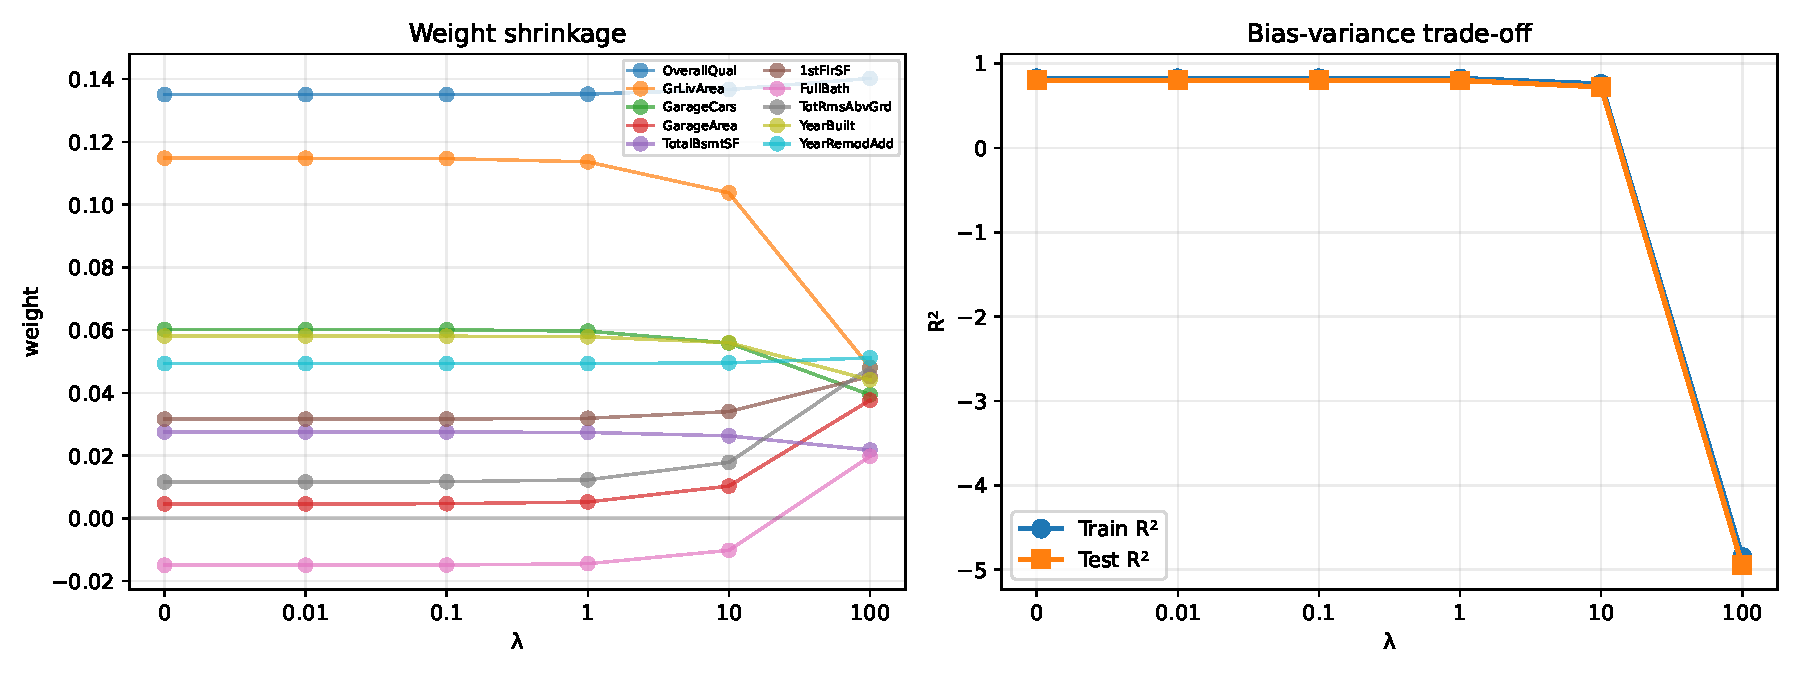
\includegraphics[width=0.7\textwidth]{ridge.pdf}

  \medskip
  \small Moderate $\lambda$ ($\leq 1$) maintains $R^2 \approx 0.80$. Large $\lambda$ over-regularises.
\end{frame}

% ============================================================
\section{PCA (Session 1)}

\begin{frame}{PCA on house features}
  \centering
  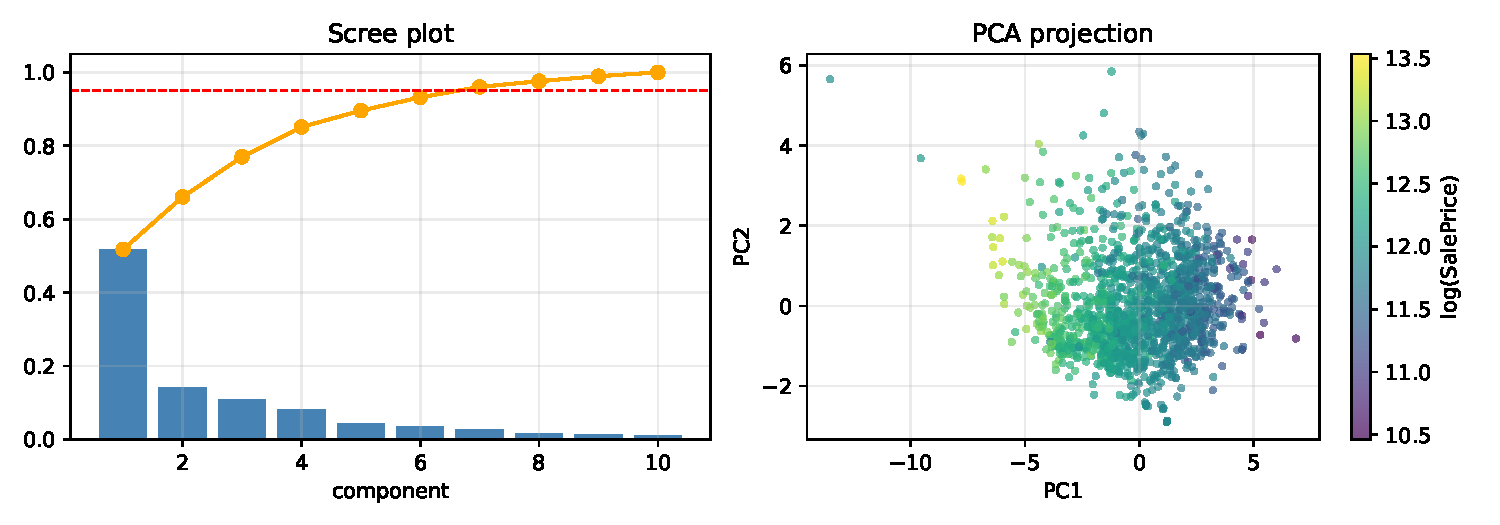
\includegraphics[width=0.78\textwidth]{pca.pdf}

  \medskip
  PC1 (52\% variance) = ``house quality'' axis. Colour confirms: PC1 sorts by price.
\end{frame}

\begin{frame}{PC loadings \& R$^2$ vs components}
  \begin{columns}[c]
    \begin{column}{0.4\textwidth}
      \centering
      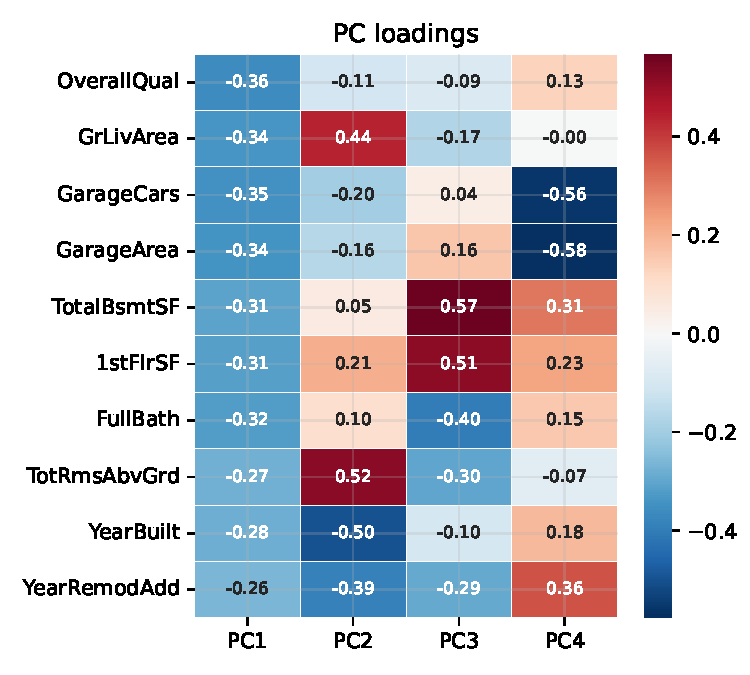
\includegraphics[width=\textwidth]{pca_loadings.pdf}
    \end{column}
    \begin{column}{0.55\textwidth}
      \centering
      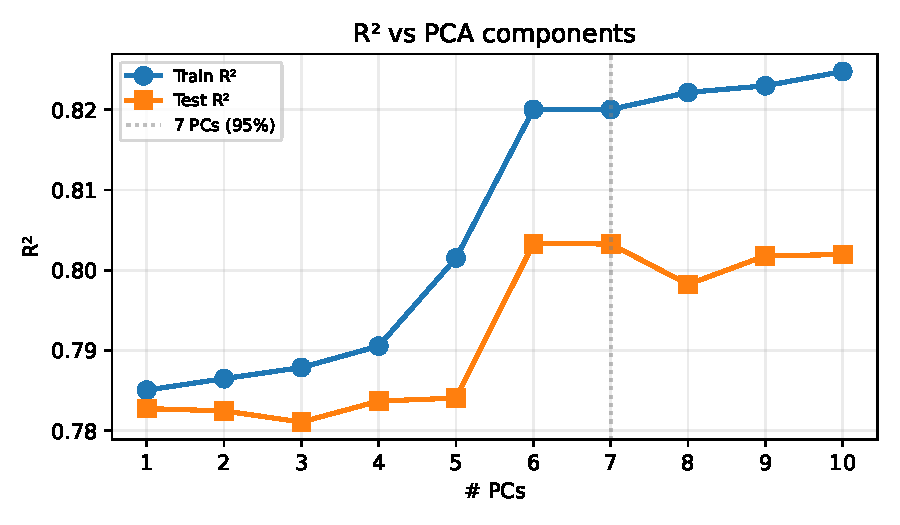
\includegraphics[width=0.85\textwidth]{pca_r2.pdf}

      \medskip
      \small 7 of 10 PCs capture 95\% variance.\\
      Top-7 PCs: $R^2 = 0.803$ vs all-features $0.802$.\\
      30\% dimensionality reduction with $<0.2\%$ $R^2$ loss.
    \end{column}
  \end{columns}
\end{frame}

% ============================================================
\section{Conclusions}

\begin{frame}{Key takeaways}
  \begin{enumerate}
    \item \textbf{GD matches OLS} to $10^{-15}$ precision with the right $\alpha$.
    \medskip
    \item \textbf{Hessian eigenvalue bound} $\alpha < 2/\lambda_{\max}$ predicts divergence --- eigenvalues (S1) govern optimisation (S2).
    \medskip
    \item \textbf{Standardisation} compressed $\kappa$ by orders of magnitude.
    \medskip
    \item \textbf{PCA} achieves 30\% reduction with minimal $R^2$ loss.
    \medskip
    \item \textbf{Ridge} offers a natural GD extension for complexity control.
  \end{enumerate}

  \medskip
  \small
  \begin{tabular}{lll}
    \toprule
    Session & Concept & Application \\
    \midrule
    1 --- Linear Algebra & Eigenvalues, PCA, $X^\top X$ & OLS, Hessian, PCA \\
    2 --- Calculus & Gradient, chain rule & GD update, LR bound \\
    3 --- Probability & Distributions & Log-transform, Q-Q \\
    4 --- Statistics & Hypothesis testing & Welch's $t$-test \\
    5 --- Advanced & Regularisation & Ridge GD \\
    \bottomrule
  \end{tabular}
\end{frame}

% ============================================================
\begin{frame}[plain]
  \centering
  \vfill
  {\Huge\textcolor{albert}{Questions?}}
  \vfill
\end{frame}

\end{document}
